% Options for packages loaded elsewhere
\PassOptionsToPackage{unicode,linktoc=none}{hyperref}
\PassOptionsToPackage{hyphens}{url}
%
\documentclass[
  letterpaper,
]{krantz}

\usepackage{amsmath,amssymb}
\usepackage{iftex}
\ifPDFTeX
  \usepackage[T1]{fontenc}
  \usepackage[utf8]{inputenc}
  \usepackage{textcomp} % provide euro and other symbols
\else % if luatex or xetex
  \usepackage{unicode-math}
  \defaultfontfeatures{Scale=MatchLowercase}
  \defaultfontfeatures[\rmfamily]{Ligatures=TeX,Scale=1}
\fi
\usepackage{lmodern}
\ifPDFTeX\else  
    % xetex/luatex font selection
\fi
% Use upquote if available, for straight quotes in verbatim environments
\IfFileExists{upquote.sty}{\usepackage{upquote}}{}
\IfFileExists{microtype.sty}{% use microtype if available
  \usepackage[]{microtype}
  \UseMicrotypeSet[protrusion]{basicmath} % disable protrusion for tt fonts
}{}
\makeatletter
\@ifundefined{KOMAClassName}{% if non-KOMA class
  \IfFileExists{parskip.sty}{%
    \usepackage{parskip}
  }{% else
    \setlength{\parindent}{0pt}
    \setlength{\parskip}{6pt plus 2pt minus 1pt}}
}{% if KOMA class
  \KOMAoptions{parskip=half}}
\makeatother
\usepackage{xcolor}
\setlength{\emergencystretch}{3em} % prevent overfull lines
\setcounter{secnumdepth}{5}
% Make \paragraph and \subparagraph free-standing
\ifx\paragraph\undefined\else
  \let\oldparagraph\paragraph
  \renewcommand{\paragraph}[1]{\oldparagraph{#1}\mbox{}}
\fi
\ifx\subparagraph\undefined\else
  \let\oldsubparagraph\subparagraph
  \renewcommand{\subparagraph}[1]{\oldsubparagraph{#1}\mbox{}}
\fi


\providecommand{\tightlist}{%
  \setlength{\itemsep}{0pt}\setlength{\parskip}{0pt}}\usepackage{longtable,booktabs,array}
\usepackage{calc} % for calculating minipage widths
% Correct order of tables after \paragraph or \subparagraph
\usepackage{etoolbox}
\makeatletter
\patchcmd\longtable{\par}{\if@noskipsec\mbox{}\fi\par}{}{}
\makeatother
% Allow footnotes in longtable head/foot
\IfFileExists{footnotehyper.sty}{\usepackage{footnotehyper}}{\usepackage{footnote}}
\makesavenoteenv{longtable}
\usepackage{graphicx}
\makeatletter
\def\maxwidth{\ifdim\Gin@nat@width>\linewidth\linewidth\else\Gin@nat@width\fi}
\def\maxheight{\ifdim\Gin@nat@height>\textheight\textheight\else\Gin@nat@height\fi}
\makeatother
% Scale images if necessary, so that they will not overflow the page
% margins by default, and it is still possible to overwrite the defaults
% using explicit options in \includegraphics[width, height, ...]{}
\setkeys{Gin}{width=\maxwidth,height=\maxheight,keepaspectratio}
% Set default figure placement to htbp
\makeatletter
\def\fps@figure{htbp}
\makeatother
\newlength{\cslhangindent}
\setlength{\cslhangindent}{1.5em}
\newlength{\csllabelwidth}
\setlength{\csllabelwidth}{3em}
\newlength{\cslentryspacingunit} % times entry-spacing
\setlength{\cslentryspacingunit}{\parskip}
\newenvironment{CSLReferences}[2] % #1 hanging-ident, #2 entry spacing
 {% don't indent paragraphs
  \setlength{\parindent}{0pt}
  % turn on hanging indent if param 1 is 1
  \ifodd #1
  \let\oldpar\par
  \def\par{\hangindent=\cslhangindent\oldpar}
  \fi
  % set entry spacing
  \setlength{\parskip}{#2\cslentryspacingunit}
 }%
 {}
\usepackage{calc}
\newcommand{\CSLBlock}[1]{#1\hfill\break}
\newcommand{\CSLLeftMargin}[1]{\parbox[t]{\csllabelwidth}{#1}}
\newcommand{\CSLRightInline}[1]{\parbox[t]{\linewidth - \csllabelwidth}{#1}\break}
\newcommand{\CSLIndent}[1]{\hspace{\cslhangindent}#1}

\usepackage{booktabs}
\usepackage{caption}
\usepackage{longtable}
\usepackage{makeidx}
\makeindex
\makeatletter
\@ifpackageloaded{tcolorbox}{}{\usepackage[skins,breakable]{tcolorbox}}
\@ifpackageloaded{fontawesome5}{}{\usepackage{fontawesome5}}
\definecolor{quarto-callout-color}{HTML}{909090}
\definecolor{quarto-callout-note-color}{HTML}{0758E5}
\definecolor{quarto-callout-important-color}{HTML}{CC1914}
\definecolor{quarto-callout-warning-color}{HTML}{EB9113}
\definecolor{quarto-callout-tip-color}{HTML}{00A047}
\definecolor{quarto-callout-caution-color}{HTML}{FC5300}
\definecolor{quarto-callout-color-frame}{HTML}{acacac}
\definecolor{quarto-callout-note-color-frame}{HTML}{4582ec}
\definecolor{quarto-callout-important-color-frame}{HTML}{d9534f}
\definecolor{quarto-callout-warning-color-frame}{HTML}{f0ad4e}
\definecolor{quarto-callout-tip-color-frame}{HTML}{02b875}
\definecolor{quarto-callout-caution-color-frame}{HTML}{fd7e14}
\makeatother
\makeatletter
\makeatother
\makeatletter
\@ifpackageloaded{bookmark}{}{\usepackage{bookmark}}
\makeatother
\makeatletter
\@ifpackageloaded{caption}{}{\usepackage{caption}}
\AtBeginDocument{%
\ifdefined\contentsname
  \renewcommand*\contentsname{Table of contents}
\else
  \newcommand\contentsname{Table of contents}
\fi
\ifdefined\listfigurename
  \renewcommand*\listfigurename{List of Figures}
\else
  \newcommand\listfigurename{List of Figures}
\fi
\ifdefined\listtablename
  \renewcommand*\listtablename{List of Tables}
\else
  \newcommand\listtablename{List of Tables}
\fi
\ifdefined\figurename
  \renewcommand*\figurename{Figure}
\else
  \newcommand\figurename{Figure}
\fi
\ifdefined\tablename
  \renewcommand*\tablename{Table}
\else
  \newcommand\tablename{Table}
\fi
}
\@ifpackageloaded{float}{}{\usepackage{float}}
\floatstyle{ruled}
\@ifundefined{c@chapter}{\newfloat{codelisting}{h}{lop}}{\newfloat{codelisting}{h}{lop}[chapter]}
\floatname{codelisting}{Listing}
\newcommand*\listoflistings{\listof{codelisting}{List of Listings}}
\makeatother
\makeatletter
\@ifpackageloaded{caption}{}{\usepackage{caption}}
\@ifpackageloaded{subcaption}{}{\usepackage{subcaption}}
\makeatother
\makeatletter
\makeatother
\ifLuaTeX
  \usepackage{selnolig}  % disable illegal ligatures
\fi
\IfFileExists{bookmark.sty}{\usepackage{bookmark}}{\usepackage{hyperref}}
\IfFileExists{xurl.sty}{\usepackage{xurl}}{} % add URL line breaks if available
\urlstyle{same} % disable monospaced font for URLs
% Make links footnotes instead of hotlinks:
\DeclareRobustCommand{\href}[2]{#2\footnote{\url{#1}}}
\hypersetup{
  pdftitle={Models},
  pdfauthor={Michael Clark \& Seth Berry},
  hidelinks,
  pdfcreator={LaTeX via pandoc}}

\title{Models}
\author{Michael Clark \& Seth Berry}
\date{}

\begin{document}
\maketitle
\renewcommand*\contentsname{Contents}
{
\setcounter{tocdepth}{2}
\tableofcontents
}
\bookmarksetup{startatroot}

\hypertarget{preface}{%
\chapter*{Preface}\label{preface}}
\addcontentsline{toc}{chapter}{Preface}

\markboth{Preface}{Preface}

Hi there, this is our book!

\hypertarget{acknowledgments}{%
\section*{Acknowledgments}\label{acknowledgments}}
\addcontentsline{toc}{section}{Acknowledgments}

\markright{Acknowledgments}

A lot of people helped when writing the book, like Gordon Ramsey,
zefrank1, and the guy who invented the wheel.

\bookmarksetup{startatroot}

\hypertarget{introduction}{%
\chapter{Introduction}\label{introduction}}

Regardless of background, and whether we're conscious of it or not, we
are constantly inundated with data. It's inescapable, from our first
attempts to understand the world around us, to our most recent efforts
to explain why we still don't get it. Even now, our most complicated and
successful models are almost uninterpretable even to those that created
them. But that doesn't mean that even in those cases we can't understand
the essence of how they work. And if you're reading this, you are
probably the type of person that wants to keep trying! So for seasoned
professionals or perhaps just the data curious, we want to help you
learn more about how to use data to answer the questions you have.

\hypertarget{what-is-this-book}{%
\section{What Is This Book?}\label{what-is-this-book}}

This book is a practical resource, something we hope you can refer to
for a quick overview of a specific modeling technique, a reminder of
something you've seen before, or perhaps a sneak peak into some modeling
details. The text is focused on a few statistical and machine learning
approaches that are widely employed, and specifically those which form
the basis for most other models in use. Believe it or not, whether a
lowly \emph{t}-test or a complex neural network, there is a tie that
binds. We hope to help you understand some of the core modeling
principles, and how the simpler models can be extended and applied to a
wide variety of data scenarios.

Our approach here is first and foremost a practical one, as models
themselves are just tools to help us reach a goal. If a model doesn't
work in the world, it's not very useful. But modeling is often a
delicate balance of interpretation and prediction, and each data
situation is unique in some way, requiring a bespoke approach. What
works well in one setting may be poor in another, and what may be the
state of the art may only be marginally better than a notably simpler
approach that is far more interpretable. In addition, complexities arise
even in an otherwise deceptively simple application. However, if you
have the core understanding of the techniques that lie at the heart of
many models, you'll automatically have many more tools at your disposal
to tackle the problems you face, and be more comfortable with choosing
the best for your needs.

\hypertarget{who-should-use-this-book}{%
\section{Who Should Use This Book?}\label{who-should-use-this-book}}

This book is intended for every type of \emph{data dabbler}, no matter
what part of the data world you call home. If you consider yourself a
data scientist, a business analyst, or a statistical hobbyist, you
already know that the best part of a good dive into data is the
modeling. But whatever your data persuasion, models give us the
possibility to answer questions, make predictions, and understand what
we're interested in a little bit better. And no matter who you are, it
isn't always easy to understand \emph{how the models work}. Even when
you do get a good grasp of a modeling approach, it can still get
complicated, and there are a lot of details to keep track of. In other
cases, maybe you just have other things going on in your life and have
forgotten a few things. We find that it's always good to remind yourself
of the basics! So if you're just interested in data and hoping to
understand it a little better, then it's likely you'll find something
useful in this book!

Your humble authors have struggled mightily themselves throughout the
course of their data history, and still do! We were initially taught by
those that weren't exactly experts, and often found it difficult to get
a good grasp of statistical modeling and machine learning. We've had to
learn how to use the tools, how to interpret the results, and possibly
the most difficult, how to explain what we're doing to others! We've
forgotten a lot, confused ourselves, and made some happy accidents in
the process. That's okay! Our goal here is to help you avoid some of
those pitfalls, help you understand the basics of how models work, and
get a sense of how most modeling endeavors have a lot of things in
common.

Whether you enthusiastically pour over formulas and code, or prefer to
skip over them, we promise that you don't need to memorize a formula to
get a good understanding of modeling and related issues. We are the
first to admit that we have long dumped the ability to pull formulas out
of our brain folds\footnote{We actually never had this ability.};
however, knowing how those individual pieces work together only helps to
deepen your understanding of the model. Typically using code puts the
formula into more concrete terms that you can then use in different ways
to solidify and expand your knowledge. Sometimes you just need a
reminder or want to see what function you'd use. And often, the
visualization will reveal even more about what's going than the formula
or the code. In short, there are a lot of tools at your disposal to help
learn modeling in a way that works for you. We hope that anyone that
would be interested in the book will find a way to learn things in a
manner that suits them best.

There is bit of a caveat. We aren't going to teach you basic statistics
or how to program in R or Python. Although there is a good chance you
will learn some of it here, you'll have an easier time if you have a
very basic understanding of statistics and some familiarity with coding.
We will provide some resources for you to learn more about these topics,
but we won't be covering them in detail. The (\textbf{appendix?}) will
provide some more information about prerequisites or just stuff that
would be good to know. However, we really aren't assuming a lot of
conceptual knowledge, and are, if anything, assuming that whatever
knowledge you have may be a bit loose or fuzzy. That's okay!

\hypertarget{what-can-you-expect}{%
\section{What Can You Expect?}\label{what-can-you-expect}}

For each model that we cover, you can expect the following in terms of
content:

\begin{itemize}
\tightlist
\item
  Overview

  \begin{itemize}
  \tightlist
  \item
    Why it's useful
  \item
    Conceptual example and interpretation
  \item
    Where the model lies in the grand scheme of topics that we will
    cover
  \end{itemize}
\item
  Key ideas and concepts

  \begin{itemize}
  \tightlist
  \item
    Brief summary and definition list of concepts or terms
  \end{itemize}
\item
  Demonstration with data, code, results, and visualizations

  \begin{itemize}
  \tightlist
  \item
    The data will often be simulations as that opens doors for further
    understanding, or a dataset that hopefully is a little more
    interesting than mtcars or iris.
  \item
    The demonstrations will provide you the opportunity to get your
    hands as dirty as you wish. We will present the code in two ways:

    \begin{itemize}
    \tightlist
    \item
      standard functions (e.g., \texttt{lm} in R, \texttt{ols} in
      \texttt{statsmodels} for Python)
    \item
      the steps to recreate the estimation process on your own (or at
      least something a little more hands-on)
    \end{itemize}
  \end{itemize}
\item
  Commentary, cautions, and where to explore next
\end{itemize}

We are taking this approach for one reason: so that you can go as deep
as you wish. If you are looking for a quick tutorial on helpful models,
then you might not find yourself going any deeper than the standard
functions (or even getting into the code at all). If you want to really
dive into these models, then you might find yourself working through the
complete steps. Another approach is to allow yourself some time between
the standard functions and complete steps. You could work through the
standard functions of every chapter, give it some time to marinate, and
then work back through the complete steps. While we certainly recommend
working through the chapters in order, we want to give you the
flexibility to choose your own depth within each.

We hope that this book can serve as a ``choose your own adventure''
statistical reference. Whether you want a surface-level understanding, a
deeper dive, or just want to be able to understand what the analysts in
your organization are talking about, you will find value in this book.
While we assume that you have a basic familiarity with coding, that
doesn't mean that you need to work through every line of code to
understand the fundamental principles and use cases of every model.

\hypertarget{which-language}{%
\section{Which Language?}\label{which-language}}

You've probably noticed most books, blogs, and courses on data science
choose R or Python. While many individuals often take an opinionated
approach towards teaching and using one over the other, we eschew
dogmatic approaches and language flame wars. R and Python are both great
languages (and equally flawed in unique ways), and it is advantageous to
be knowledgeable of both, even if you focus on one specifically, as they
are the most popular languages for statistical modeling and machine
learning. We use both extensively in our own work for teaching, personal
use, and production level code, and have found both are up to whatever
task you have in mind. Throughout this book, we will be presenting
demonstrations in both R and Python, and you can use both or take your
pick, but we want to leave that choice up to you. Our goal isn't to
obscure the ideas behind packages and specialty functions or tell you
why one languages is superior to the other (they aren't), but to show
you the most basic functions behind big model ideas.

While we want to provide you choice, we truly hope that displaying both
languages can help people to ``convert'' from one to the other. We have
spent countless hours, slumped over our computers, debugging errors and
figuring things out. If we can take away one source of pain for you,
that would be great! We'd like to consider this as a resource for the R
user, who knows exactly what they want to do in R, but could use a
little help translating their R knowledge to Python; we'd also like this
book to be a resource for the Python user, who sees the value in R's
statistical modeling abilities.

\hypertarget{choose-your-own-adventure}{%
\section{Choose Your Own Adventure}\label{choose-your-own-adventure}}

As an example of how things will go, let's look at the different ways we
might express a relationship between two variables. If you want just a
little bit of background, you can read through the \emph{Overview} and
\emph{Key Ideas}. If you want to see the easy way to use the model, you
can work through the \emph{Standard Function} section. If you want to
see the method from start to finish, feel free to work through the
\emph{Roll Your Own} section. If all of that sounds like a lot of work
and you'd rather look at the pretty pictures, that's fine
too\footnote{We love pretty pictures too! Sometimes it's the best way to
  bring a lot of ideas together.}, just jump to the \emph{Visualization}
section.

\hypertarget{overview}{%
\subsection{Overview}\label{overview}}

Correlations provide a means of understanding how, and \emph{if}, two or
more things are related. For any two variables or features, we can
estimate a single value that signals the strength and direction of the
relationship between them. Despite limitations, correlations can be a
great way to get a quick understanding of the relationship between two
features. One variable could be temperature while another variable is
the number of ice cream cones sold, or one is the number of hours spent
studying and another variable is the grade on a test, maybe the number
of hours spent watching TV versus the number of hours spent exercising.
The correlation value will give us information that is similarly
interpretable in each case.

\hypertarget{key-ideas}{%
\subsection{Key Ideas}\label{key-ideas}}

Here are key ideas to consider for understanding correlation.

\begin{itemize}
\tightlist
\item
  \textbf{Variance}: Two variables must vary if they are to
  \emph{co-}vary
\item
  \textbf{Covariance}: Joint variability of two variables, i.e.~how they
  vary together
\item
  \textbf{Interpretation}: Covariance is hard to interpret because the
  variables are typically on different scales
\item
  \textbf{Correlation}: Correlation is a standardized covariance, so it
  is easier to interpret
\end{itemize}

Another way to think about correlation is through the lens of
\emph{variance} \emph{covariance}. Covariance is a measure of the joint
variability of two variables, i.e.~how they \emph{vary} together. If two
variables are highly correlated, then they have a high degree of
covariance, i.e.~they vary together in a meaningful way.

\hypertarget{demonstration}{%
\subsection{Demonstration}\label{demonstration}}

To demonstrate correlation, we could start by formally defining it. Here
is a formula for the Pearson-Product-Moment correlation coefficient.
What everyone typically just calls ``correlation'' or Pearson's \emph{r}
is actually the \emph{Pearson Product-Moment Correlation} -- that is a
lot of words, though, so we will just go with correlation. As we
mentioned earlier, we want to give you the choice to dive in as deep as
you want.

\begin{equation}\protect\hypertarget{eq-pearson}{}{
\rho = \frac{\Sigma(x_i-\bar{x})(y_i-\bar{y})}{\sqrt{\Sigma(x_i-\bar{x})^2\Sigma(y_i-\bar{y})^2}}
}\label{eq-pearson}\end{equation}

In words, starting with the numerator, we are going to subtract the mean
of \emph{x} from every observation of \emph{x}, do the same for
\emph{y}, multiply them together, and then sum them to produce a single
value. If you've taken a statistics class before, you might have seen
this part of the formula when talking about \emph{covariance} -- the
joint variability of two variables. In fact, if you just divide the
numerator by n-1 you'd get the covariance value. Covariance values,
though, are not standardized; therefore, they are a bit tough to
interpret. You will get a sign indicating relationship (just like a
correlation) and the magnitude tells you the strength of the
relationship, but it is hard to get your head around how much stronger a
covariance of 4.00 is compared to a covariance of 0.28.

This is where the denominator comes into play. To put it into real
terms, we will subtract the mean of \emph{x} from every observation of
\emph{x} (i.e.~get the deviations of x), square those values, and sum
those values to produce a single value. We will do the same for
\emph{y}, multiply those results, and then take the square root of that
product. The denominator might also look familiar to some. The
individual pieces- \(\Sigma(x_i-\bar{x})^2\) and
\(\Sigma(y_i-\bar{y})^2\) - are computing the \emph{variance} of x and
y. Taking the square root of variance gives us the \emph{standard
deviation}. Basically, we're getting a combined standard deviation to
scale the covariance. Using the standard deviation will mitigate the
effects of \emph{x} and \emph{y} potentially being on different scales;
in other words, we want to know how much two variables move together,
even if the means and typical movement (deviation) might be very
different.

Here is a simplification, depicting correlation as a
\textbf{standardized covariance}.

\begin{equation}\protect\hypertarget{eq-corcov}{}{
\rho = \frac{cov(x,y)}{\sigma_x\sigma_y}
}\label{eq-corcov}\end{equation}

where \(cov(x,y)\) is the covariance between \(x\) and \(y\), and
\(\sigma_x\) and \(\sigma_y\) are the standard deviations of \(x\) and
\(y\), respectively. So putting it all together, we are simply looking
at the ratio of raw covariance (i.e., how much two variables ``move''
together) and standard deviation (i.e., the amount of dispersion within
a variable). Just as we mentioned earlier, simpler concepts often tie
models together! What might look like a tricky formula, really just
starts with means and deviations, variance and covariance!

As a reminder, this correlation will give us an idea about the
\textbf{linear relationship} between two continuous variables; we will
get a value between -1 and 1, with values closer to 0 indicating that
there is no linear relationship between the two variables. As values get
closer to 1, we have a \textbf{positive correlation} -- as values for
one variable increase, values for the other variable tend to increase
along with it. As the correlation gets closer to -1, we have a
\textbf{negative correlation} -- as values for one variable increase,
values for the other variable typically decrease. Correlations can be
useful for quickly exploring linear relationships, but let's not get too
excited about it -- they aren't going to help you answer any big
questions! We also don't want to get too carried away with ``statistical
significance'' yet -- once samples get large, even small correlations
become ``significant''. Instead, just use correlations to explore the
patterns within your data, start getting ideas about interesting
relationships that you might find, and leave worries about significance
for people with more time on their hands.

\hypertarget{code}{%
\subsubsection{Code}\label{code}}

It's often easier to understand a concept by seeing it in action. So
let's start by creating some data. We'll create a variable \texttt{x},
then make a \texttt{y} that will have a linear relationship with it, but
also have some random noise. We'll then plot the two variables to see
what they look like. To help your understanding, fiddle with the knobs
noted.

\subsubsection{R}

\begin{verbatim}
set.seed(seed = 1001)
N <- 500
x <- rnorm(n = N, mean = 0, sd = 1)

# Fiddle with the .5 and .75.
# The first can also be negative if you like!
y <- .5 * x + rnorm(n = N, mean = 0, sd = .75)
\end{verbatim}

\subsubsection{Python}

\begin{verbatim}
import numpy as np

np.random.seed(seed = 1001)
N = 500
x = np.random.normal(loc = 0, scale = 1, size = N)

# Fiddle with the .5 and .75. 
# The first can also be negative if you like!
y = .5*x + np.random.normal(loc = 0, scale = .75, size = N) 
\end{verbatim}

Now check out the plot of those two values:

\begin{figure}

{\centering 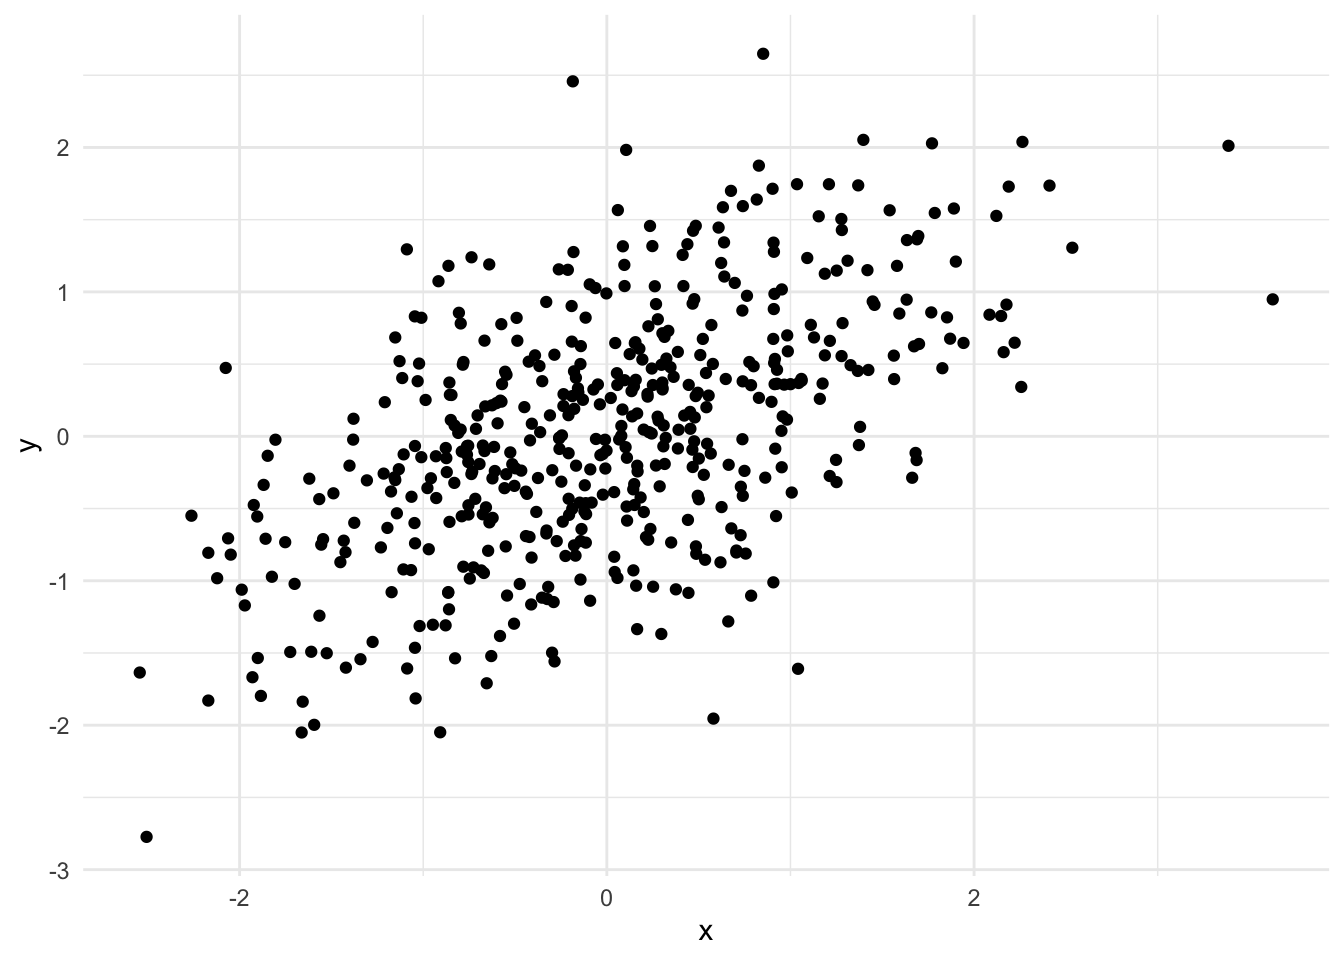
\includegraphics{introduction_files/figure-pdf/cor_viz-1.pdf}

}

\caption{Scatterplot of two variables.}

\end{figure}

Remember that correlation is testing for the presence of a linear
relationship, with -1 indicating a perfect negative relationship, 1
indicating a perfect positive relationship, and 0 indicating no
relationship. Before we see the actual correlation value for these two
variables, take a guess as to what value we are going to get!

Before we create our own function, we can use R's \texttt{cor} function
or numpy's \texttt{corrcoef} function. You should get something around
0.6.

\begin{verbatim}
# Results for R and Python will be slightly
# different due to different random number generators
cor(x, y)
np.corrcoef(x, y)
\end{verbatim}

\begin{verbatim}
[1] 0.557
\end{verbatim}

When you guessed the value, were you close? If so, congrats! If not, try
fiddling with those knobs noted until things get a little clearer. But
now that we already know the answer, let's make sure that we can get the
same answer by working through the formula via code. The following takes
that initial formula approach and turns it into a function that we can
use to compute the correlation between any two variables. We'll then use
that function to compute the correlation between our \texttt{x} and
\texttt{y} variables.

\subsubsection{R}

\begin{verbatim}
my_cor = function(x, y) {
    # First, we need to compute the averages for x and y.
    # The rest follows the formula.
    x_bar = mean(x)
    y_bar = mean(y)

    numerator = sum((x - x_bar) * (y - y_bar))

    denominator = sqrt(
        sum((x - x_bar)^2) * sum((y - y_bar)^2)
    )

    numerator / denominator
}

# using the builtin functions
my_cor2 = function(x, y) {
    cov(x, y) / (sd(x) * sd(y))
}

my_cor(x, y)
\end{verbatim}

\begin{verbatim}
[1] 0.557
\end{verbatim}

\subsubsection{Python}

\begin{verbatim}
def my_cor(x, y):
  # First, we need to compute the averages for x and y.
  # The rest follows the formula.
    x_bar = np.mean(x)
    y_bar = np.mean(y)
    
    numerator = np.sum((x - x_bar) * (y - y_bar))
    
    denominator = np.sqrt(
      np.sum((x - x_bar)**2) * np.sum((y - y_bar)**2)
    )

    # We will finish by dividing the numerator by the 
    # denominator.
    # This will ensure that we have a value between -1 and 1.
    return(numerator / denominator)

my_cor(x, y)
\end{verbatim}

\begin{verbatim}
0.5390318454354402
\end{verbatim}

It doesn't matter which language we use, the steps are largely the same
when we break it down into the individual pieces!

\hypertarget{visualization}{%
\subsection{Visualization}\label{visualization}}

A long time ago, in a land far away, the authors of this book worked
together to help clients traverse the forests of data to reach their
modeling goals. While there were many great learning opportunities along
the way, working with clients showed us the kinds of help that people
really needed in adventuring with data and models. Even so, there were
many requests that made us grimace, and one stood atop Mount Ridiculous:
to produce a correlation matrix with 115 variables and export that
matrix to a spreadsheet. We still don't recommend such shenanigans, but
there are ways to try and understand correlation matrices. Since we were
in the business of helping people do their work better, one way we often
did so was via a \emph{corrplot}.

We'll start with a something manageable. We create a data set with six
variables of two sets: a, b , c, and x, y, z, and then we can take a
quick look at the correlation matrix.

\begin{longtable}{lrrrrrr}
\caption{Correlation matrix}\tabularnewline

\toprule
feature & a & b & c & x & y & z \\ 
\midrule
a & $1.00$ & $0.47$ & $0.45$ & $-0.24$ & $-0.17$ & $-0.13$ \\ 
b & $0.47$ & $1.00$ & $0.51$ & $-0.18$ & $-0.16$ & $-0.07$ \\ 
c & $0.45$ & $0.51$ & $1.00$ & $-0.25$ & $-0.20$ & $-0.14$ \\ 
x & $-0.24$ & $-0.18$ & $-0.25$ & $1.00$ & $0.51$ & $0.45$ \\ 
y & $-0.17$ & $-0.16$ & $-0.20$ & $0.51$ & $1.00$ & $0.49$ \\ 
z & $-0.13$ & $-0.07$ & $-0.14$ & $0.45$ & $0.49$ & $1.00$ \\ 
\bottomrule
\end{longtable}

Now we have the \emph{pairwise correlations} between all six of our
variables, with 1's on the diagonals (naturally, a variable has a
perfect correlation with itself). You can check out the lower diagonal
or the upper diagonal, because they contain the exact same information.
Quickly, though, find the interesting pattern in that matrix!

Producing the correlations between just 6 variables gives us 15
correlation coefficients to examine! You can see that you'll need to
spend more than a few seconds on finding the interesting patterns within
the data (or if there are any patterns at all). Our brains are oriented
towards vision, so we can use \emph{preattentive processing} elements,
like hue, saturation, and size, to make finding interesting patterns
easier.

Since we already have a correlation matrix, we can use various means to
find those patterns, which include visualizing the matrix itself,
network graphs and others. Here is one way to do it.

\begin{tcolorbox}[enhanced jigsaw, coltitle=black, title=\textcolor{quarto-callout-note-color}{\faInfo}\hspace{0.5em}{Note}, colback=white, opacityback=0, bottomtitle=1mm, colframe=quarto-callout-note-color-frame, toptitle=1mm, bottomrule=.15mm, titlerule=0mm, leftrule=.75mm, arc=.35mm, rightrule=.15mm, toprule=.15mm, opacitybacktitle=0.6, left=2mm, colbacktitle=quarto-callout-note-color!10!white, breakable]

Some recommended R packages for visualizing a correlation matrix include
\texttt{corrr}, \texttt{ggcor}, and \texttt{corrplot}. For python, one
has options for \texttt{seaborn}, \texttt{pandas}, \texttt{biokit}, and
others.

\end{tcolorbox}

\begin{figure}

{\centering 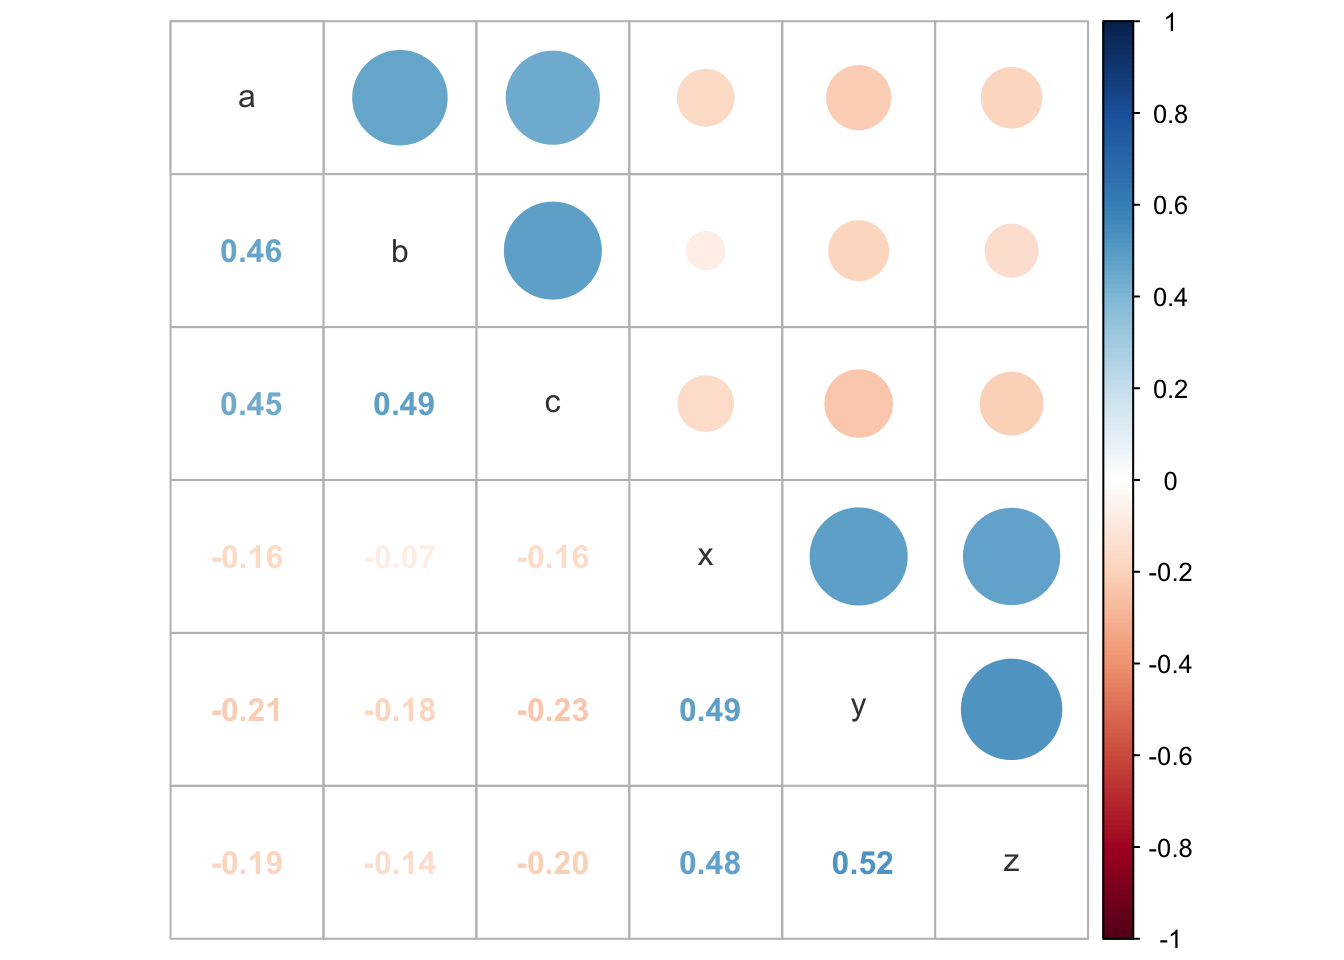
\includegraphics{introduction_files/figure-pdf/corrplot_demo-1.pdf}

}

\caption{Correlation matrix visualization}

\end{figure}

Let's break down what we're seeing just a little bit. The lower triangle
has the correlation values. It adds information, though, by changing the
hue by correlation value -- red for negative values and blue for
positive values -- and increasing the saturation as the correlation
value becomes stronger. The upper triangle contains the same
information, but the size of the circle is tied directly to the strength
of the correlation. You'll also notice that the weaker correlations are
more hidden in the visualization, allowing us to focus only on those
interesting relationships.

What do you think? Was it easier to spot the points of interest? It
looks like there is an a-b-c group and x-y-z group that are similarly
correlated within their respective groups. We can also see that the
a-b-c group is negatively correlated with the x-y-z group. Visualizing
the correlation matrix can usually make it easier to find those
interesting patterns.

\hypertarget{commentary}{%
\subsection{Commentary}\label{commentary}}

The correlation is a starting point for understanding linear models,
which serve as the foundation for modeling in general. It is very
limited by only assessing linear relationships between variables, as
well as only pairwise relationships. Other metrics can overcome these,
but they have their own limitations. The basic Pearson-Product-Moment
correlation coefficient is still the most widely used and a typical
starting point in many data adventures.

Things to explore further next:

\begin{itemize}
\tightlist
\item
  Rank correlation (e.g., Spearman's rho, Kendall's tau)
\item
  Distance metrics (e.g., euclidean, manhattan, cosine)
\item
  Non-linear relationships and interactions (e.g., distance correlation,
  polynomial, splines)
\item
  Multivariate relationships (e.g., partial correlations, r-squared)
\end{itemize}

\hypertarget{moving-towards-an-excellent-adventure}{%
\section{Moving Towards An Excellent
Adventure}\label{moving-towards-an-excellent-adventure}}

Remember the point we made about ``choosing your own adventure''?
Statistical modeling and programming is an adventure, even if you never
leave your desk! Every situation calls for choices to be made and every
choice you make will lead you down a different path. You will run into
errors, dead ends, and you might even find that you've spent
considerable time to conclude that nothing interesting is happening in
your data. This, no doubt, is part of the fun and all of those struggles
make success that much sweeter. Like every adventure, things might not
be immediately clear and you might find yourself in perilous situations!
If you find that something isn't making sense upon your first read, that
is okay. Both authors have spent considerable time mulling over models
and foggy ideas during our assorted (mis)adventures; nobody should
expect to master complex concepts on a single read through! In any arena
where you strive to develop skills, distributed practice and repetition
are essential. When concepts get tough, step away from the book, and
come back with a fresh mind.

Thanks for coming on this adventure with us and welcome to our
\emph{Book of Models}.

This is a test reference (Hastie, Tibshirani, and Friedman 2009).

\cleardoublepage
\phantomsection
\addcontentsline{toc}{part}{Appendices}
\appendix

\hypertarget{references}{%
\chapter*{References}\label{references}}
\addcontentsline{toc}{chapter}{References}

\markboth{References}{References}

\hypertarget{refs}{}
\begin{CSLReferences}{1}{0}
\leavevmode\vadjust pre{\hypertarget{ref-hastie_elements_2009}{}}%
Hastie, Trevor, Robert Tibshirani, and Jerome Friedman. 2009. \emph{The
Elements of Statistical Learning: Data Mining, Inference, and
Prediction, Second Edition}. 2nd ed. 2009. Corr. 3rd printing 5th
Printing. Springer.

\end{CSLReferences}



\printindex

\end{document}
